% Reconstructed semantic LaTeX: editable paragraphs, equations, figures and citations.

\chapter{Simulation workflow}
\label{sec:03_simulation_workflow_simulation_workflow}

Two independently generated simulation datasets are used and are not pooled into a single benchmark. The longitudinal dataset provides one-dimensional density-to-density examples for the Fourier Neural Operator (FNO). The six-dimensional dataset provides paired input– output particle clouds for the CVAE and latent-propagation models. Their numerical errors are task-specific and must not be compared directly.

\section{Six-dimensional Xsuite tracking dataset}
\label{sec:03_simulation_workflow_six_dimensional_xsuite_tracking_dataset}

The six-dimensional dataset was generated with Xsuite version 0.48.4, the latest public release available on 1 April 2026 \cite{xsuite2026documentation,iadarola2023xsuite}. Xsuite is an open-source Python suite for multiparticle accelerator simulations. In the present workflow, its Xtrack component performs macroparticle transport after the MAD-X lattice description has been imported through cpymad. The complete generation workflow is available in the public \texttt{ML4CollEffects} repository \cite{martinez2026code}, serving as the six-dimensional data-generation entry point.

For each sample \(s ,\) a parameter vector \(\mu^{( s )}\) and a sampled input beam family define the macroparticle cloud

\begin{equation}
\label{eq:34}
Z_{\mathrm{in}}^{(s)}=\left\{\xi_n^{(s)}\right\}_{n=1}^{N_p},
\end{equation}

which is tracked through the selected lattice realization to obtain

\begin{equation}
\label{eq:35}
Z_{\mathrm{out}}^{(s)}=\Phi_{\mu^{(s)}}\left(Z_{\mathrm{in}}^{(s)}\right).
\end{equation}

The resulting supervised dataset is

\begin{equation}
\label{eq:36}
\mathcal D_{\mathrm{track}}=\left\{\left(Z_{\mathrm{in}}^{(s)},\mu^{(s)},Z_{\mathrm{out}}^{(s)}\right)\right\}_{s=1}^{2048}.
\end{equation}

The working archive used for the reported models contains 2048 paired trajectories, with \(N_{p} =\) 4096 retained macroparticles in each input and output cloud. The fixed data-partition indices are stored in the arrays train, val, and test. The split contains 1640 training samples, 204 validation samples, and 204 test samples. The reference generator used a larger macroparticle population before the stored clouds were reduced to the fixed array size used by the machine-learning pipeline. The coordinate order used in the archive is

\begin{equation}
\label{eq:37}
(x,y,\zeta,p_x,p_y,\delta),
\end{equation}

which differs from the canonical plane-grouped notation \(( x , p_{x} , y , p_{y} , \zeta , \delta )\) used in parts of Chapter 2. Array indices and pairwise-histogram channels follow the ordering in Eq.~\eqref{eq:37}; this convention is stated explicitly to avoid ambiguity in the physical interpretation of the stored channels.

The optics input corresponds to the FCC-ee HEB lattice release, obtained from the public FCC-ee HEB optics archive \cite{fcc2026lattice}. The generation script imports the MAD-X driver, selects the FCC-ee HEB sequence, and converts the selected lattice section into an Xtrack line. The FCC-ee HEB wake and impedance inputs were obtained from the public FCC-ee Booster PyWIT model repository \cite{impedan2026pywit}. Since both the optics archive and the impedance model remain subject to updates, the archival dataset release will preserve the exact input files used in this work, together with their cryptographic checksums.

For component \(\mu_{k} ,\) the nominal in-distribution range is defined from the training subset only,

\begin{equation}
\label{eq:38}
I_k=\left[\min_{s\in\mathcal D_{\mathrm{train}}}\mu_k^{(s)},\max_{s\in\mathcal D_{\mathrm{train}}}\mu_k^{(s)}\right].
\end{equation}

No validity claim is made outside \(\mathcal{I}_{k k}^{Q} .\) Following the element-conditioned latent-dynamics formulation of \cite{wang2026latent}, each lattice element is described by the seven-dimensional parameter vector

\begin{equation}
\label{eq:39}
\mu_i=(L_i,K_{1,i},K_{2,i},\phi_i,V_{\mathrm{rf},i},f_{\mathrm{rf},i},\varphi_{\mathrm{rf},i})\in\mathbb R^7,
\end{equation}

where \(L_{i}\) is the element length, \(K_{1 , i}\) and \(K_{2 , i}\) are the quadrupole and sextupole strengths, \(\phi_{i}\) is the dipole bending angle, and \(V_{\mathrm{rf} , i} , f_{\mathrm{rf} , i} ,\) and \(\varphi_{\mathrm{rf} , i}\) are the RF-cavity voltage, frequency, and phase. For non-RF elements, \(V_{\mathrm{rf} , i} = f_{\mathrm{rf} , i} =\) 0.

Before embedding, each component is normalized according to its numerical scale. The RF voltage and frequency are compressed using the transformation \(x \mapsto\) log(1 \(+ x ) ,\) which reduces their large dynamic range while preserving the zero value assigned to non-RF elements. The remaining parameters are normalized as

\begin{equation}
\label{eq:40}
\begin{gathered}\widetilde L_i=\frac{L_i}{1.0\,\mathrm m},\quad\widetilde K_{1,i}=\frac{K_{1,i}}{10.0\,\mathrm m^{-2}},\quad\widetilde K_{2,i}=\frac{K_{2,i}}{10.0\,\mathrm m^{-3}},\\\widetilde\phi_i=\frac{\phi_i}{2\pi},\qquad\widetilde\varphi_{\mathrm{rf},i}=\frac{\varphi_{\mathrm{rf},i}}{2\pi}.\end{gathered}
\end{equation}

\section{PyColleff longitudinal dataset}
\label{sec:03_simulation_workflow_pycolleff_longitudinal_dataset}

The longitudinal benchmark was generated using the \texttt{pycolleff} module distributed in the LNLS collective effects repository \cite{desa2024pycolleff}. PyColleff is a Python package for impedance modelling and instability analysis in electron storage rings. In this work, it is used as a controlled operator-learning benchmark rather than as a validated end-to-end model of the FCC-ee HEB. The implemented configuration uses a \(3 ,\) GeV ring model, a uniform longitudinal grid with \(N_{\zeta} =\) 2048, a resonator contribution with quality factor \(Q =\) 104, three fixed-point relaxation steps, and an under-relaxation coefficient \(\alpha = 0.7 .\) The sampled conditioning variables are the bunch current, chamber radius, and non-evaporable-getter coating thickness. Their uniform ranges are \(I_{b} \in [ 200 ,\) 350] A, \(R \in [ 5 ,\) 12] mm, and \(t_{\mathrm{NEG}} \in [ 1 ,\) 3] \(\mu \mathrm{m} .\) These variables modify the longitudinal response and the resistive-wall and material contributions represented by the benchmark configuration.

\begin{equation}
\label{eq:41}
\mu^{(s)}=\left(I_b^{(s)},R^{(s)},t_{\mathrm{NEG}}^{(s)}\right).
\end{equation}

The induced voltage is evaluated spectrally as

\begin{equation}
\label{eq:42}
V_{\mathrm{ind}}(z)=-\mathcal F^{-1}\left[Z_{\parallel}(\omega;\mu)\widehat\lambda(\omega)\right](z),
\end{equation}

and the total voltage is

\begin{equation}
\label{eq:43}
V_{\mathrm{tot}}(z)=V_{\mathrm{RF}}(z)+V_{\mathrm{ind}}[\lambda](z).
\end{equation}

The truncated fixed-point update is

\begin{equation}
\label{eq:44}
\lambda^{(k+1)}=(1-\alpha)\lambda^{(k)}+\alpha\mathcal T_{\mu}\left(\lambda^{(k)}\right),
\end{equation}

with \(K =\) 3 iterations and \(\lambda_{\mathrm{out}} = \lambda^{( K )} .\) The resulting data are

\begin{equation}
\label{eq:45}
\mathcal D_{\lambda}=\left\{\left(\lambda_{\mathrm{in}}^{(s)},\mu^{(s)},\lambda_{\mathrm{out}}^{(s)}\right)\right\}_{s=1}^{2048}.
\end{equation}

The ranges and units of every component of \(\mu\) are therefore explicit. Reproducibility additionally requires the RF settings, impedance components, material model, boundary conventions, and PyColleff version; these items are preserved with the generation configuration so that the FNO result is not mistaken for a surrogate of a different impedance model.

\section{Data representation and physical quantities}
\label{sec:03_simulation_workflow_data_representation_and_physical_quantities}

\subsection{Empirical measures and reduced profiles}
\label{sec:03_simulation_workflow_empirical_measures_and_reduced_profiles}

A cloud defines the empirical probability measure

\begin{equation}
\label{eq:46}
\rho^{N_p}=\frac1{N_p}\sum_{n=1}^{N_p}\delta_{\xi_n}.
\end{equation}

For the longitudinal task, this measure is projected onto the uniform grid \(\{ \zeta_{j} \}_{j = 1}^{\zeta}\) to form

\begin{equation}
\label{eq:47}
\lambda^h=\bigl(\lambda(\zeta_1),\ldots,\lambda(\zeta_{N_{\zeta}})\bigr)\in\mathbb R^{N_{\zeta}}.
\end{equation}

The profile is normalized to unit integrated mass before being supplied to the FNO.

\subsection{Fifteen pairwise phase-space projections}
\label{sec:03_simulation_workflow_fifteen_pairwise_phase_space_projections}

A direct 646 discretization of the full six-dimensional density is infeasible. The tracking state is therefore represented by all fifteen pairwise two-dimensional histograms,

\begin{equation}
\label{eq:48}
\mathcal P=\{(i,j):1\le i<j\le6\},\qquad H(\rho)=\{H_{ij}\}_{(i,j)\in\mathcal P}\in\mathbb R^{15\times64\times64}.
\end{equation}

For sample \(s ,\) coordinate \(i\) is histogrammed over the sample-adaptive interval

\begin{equation}
\label{eq:49}
\left[m_i^{(s)}-5\sigma_i^{(s)},\,m_i^{(s)}+5\sigma_i^{(s)}\right],
\end{equation}

where \(m_{i}\) and \(\sigma_{i}\) are the empirical centroid and coordinate-wise RMS spread defined in Eq.~\eqref{eq:26}. Every pairwise channel is converted to a probability-mass array,

\begin{equation}
\label{eq:50}
\sum_{a=1}^{64}\sum_{b=1}^{64}H_{ij}^{(s)}[a,b]=1.
\end{equation}

Thus, the CVAE histogram branch models normalized projected shape. The six centroids and six RMS spreads are retained as a separate 12-component physical vector and provide the location and coordinate scale omitted by independent channel normalization. When a physical probability density is required, the normalized mass is divided by the physical bin area,

\begin{equation}
\label{eq:51}
\rho_{ij}^{(s)}[a,b]=\frac{H_{ij}^{(s)}[a,b]}{\Delta\xi_{i,a}^{(s)}\Delta\xi_{j,b}^{(s)}}.
\end{equation}

The word \emph{beam} \emph{size} is therefore not used for all twelve auxiliary quantities. The transverse position spreads \(\sigma_{x}\) and \(\sigma_{y}\) may be related to conventional optical beam sizes under the assumptions stated in Section 2.3.1; the remaining entries are coordinate-wise RMS spreads of \(p_{x} , p_{y} , \zeta ,\) and \(\delta .\) The RMS definition remains meaningful for non-Gaussian distributions but is not a complete shape descriptor. Non-Gaussian information is carried by the histograms, while explicit quantiles are left to future work.

Pairwise marginals do not uniquely determine a six-dimensional joint density and predicted channels need not be mutually consistent. For coordinate \(i ,\) let \(h_{i}^{( i j )}\) be the one-dimensional marginal obtained by summing \(H_{i j}\) over coordinate \(j .\) A shared-marginal consistency diagnostic is

\begin{equation}
\label{eq:52}
E_{\mathrm{cons}}=\frac16\sum_{i=1}^{6}\frac1{|\mathcal C_i|}\sum_{(ij),(ik)\in\mathcal C_i}\left\|h_i^{(ij)}-h_i^{(ik)}\right\|_1,
\end{equation}

where \(\mathcal{C}_{i}\) contains histogram channels sharing coordinate \(i .\)

The information loss can be stated more formally through an ANOVA/Hoeffding-type decomposition of a joint density,

\begin{equation}
\label{eq:53}
\begin{aligned}\rho(\xi_1,\ldots,\xi_6)&=\rho_0+\sum_i f_i(\xi_i)+\sum_{i<j}f_{ij}(\xi_i,\xi_j)\\&\quad+\sum_{i<j<k}f_{ijk}(\xi_i,\xi_j,\xi_k)+\cdots+f_{1\cdots6}(\xi_1,\ldots,\xi_6).\end{aligned}
\end{equation}

The fifteen pairwise marginals constrain one- and two-coordinate information but do not identify the three- through six-coordinate interaction terms. For a multivariate Gaussian distribution, the mean vector and covariance matrix determine the full joint density, so pairwise information is sufficient in that special case. The collective, halo-bearing, and strongly distorted distributions of interest here are not assumed to be Gaussian; omitted higher-order correlations may therefore be dynamically relevant. The reported CVAE reconstruction error measures fidelity to the fifteen-channel representation, not error with respect to the unknown complete six-dimensional density.

A direct estimate of this representation error was not retained in the present experiments. Such a test would require a model that can evaluate or sample a six-dimensional joint density and then compare observables that depend on three or more coordinates. Point-cloud generative models and maximum-entropy normalizing-flow tomography provide natural alternatives because they represent a joint six-dimensional distribution without a 646 grid \cite{hoover2024tomography}. A controlled comparison against one of these alternatives, including halo-rich and strongly distorted cases, is therefore a priority for future work rather than a result claimed here.

\section{Computational cost}
\label{sec:03_simulation_workflow_computational_cost}

Table 4 reports exploratory generation timings recorded for the reference pipeline. They depend on hardware, parallelization, numerical precision, cache state, and software versions. The measurements were not obtained under one final hardware-normalized protocol and are therefore not used as a controlled simulator-versus-network benchmark; they document only the order of magnitude of data generation. The tracking timing corresponds to the reference high-particle-count generator, whereas the stored machine-learning archive contains 4096 retained macroparticles per cloud.

\begin{figure}[!htbp]
\centering
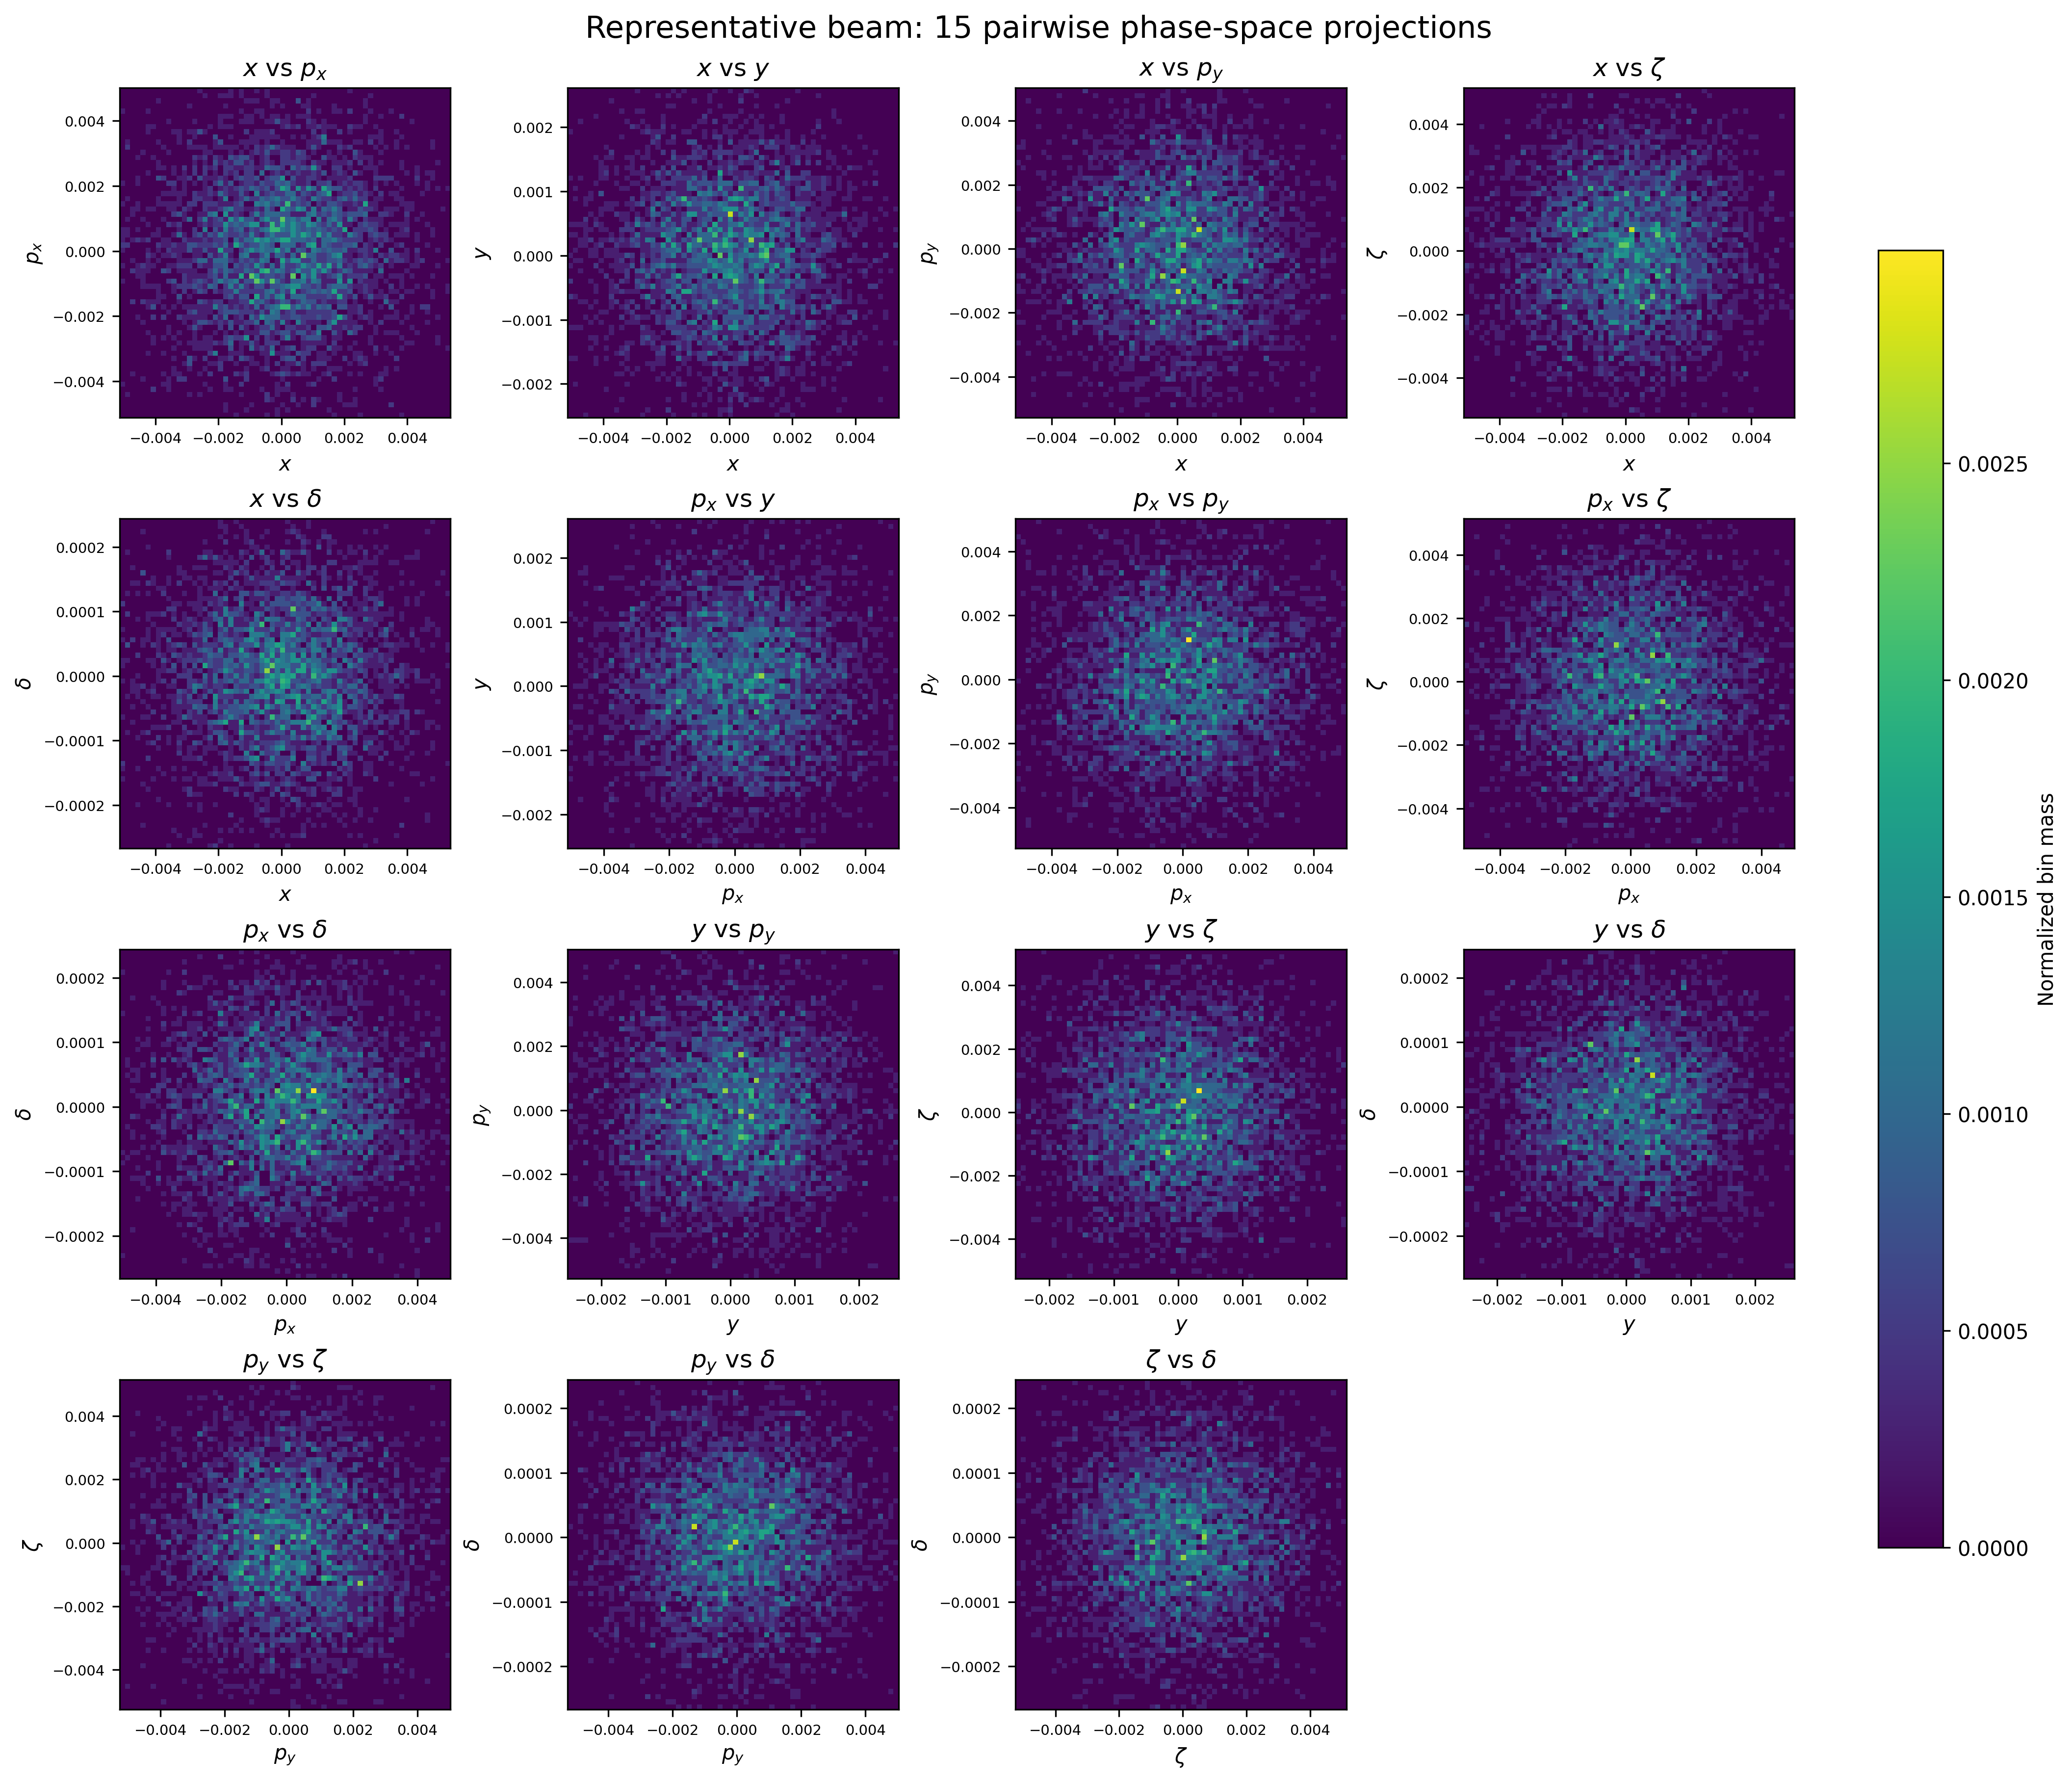
\includegraphics[width=1.0000\linewidth]{beam_pairwise_phase_space_marginals.png}
\caption{Representative beam state encoded through its fifteen pairwise two-dimensional phase-space marginals. The associated centroid and coordinate-wise RMS-spread vectors retain complementary information about physical position and extension. The figure represents a reduced description of a six-dimensional state, not a unique reconstruction of the complete joint density.}
\label{fig:beam_pairwise_phase_space_marginals}
\end{figure}

\begin{table}[!htbp]
\centering\small
\caption{Exploratory computational cost recorded for the reference pipeline. “Particles/grid” denotes macroparticles for tracking and histogram generation, and longitudinal grid points for PyColleff.}
\label{tab:4}
\begin{adjustbox}{max width=\linewidth}
\begin{tabular}{lrrrc}\toprule
Data source & Samples & Particles/grid & Time/sample [s] & Total [s]\\\midrule
Xsuite tracking & 2048 & $10^6$ particles & 1.41 & 2904.52\\
PyColleff longitudinal solver & 2048 & 2048 grid points & 2.72 & 5568.32\\
6D histogram generation & 2048 & $10^6$ particles & $2.32\times10^{-3}$ & 4.75\\\bottomrule\end{tabular}
\end{adjustbox}
\end{table}

ence time of \(2.338\) ms per sample gives the nominal ratio

\begin{equation}
\label{eq:54}
\frac{1.41\,\mathrm s}{2.338\times10^{-3}\,\mathrm s}\simeq603.
\end{equation}

This approximately \(600 \times\) ratio is useful for indicating the potential order of magnitude, but it is not reported as a controlled speed-up because the simulator and neural timings were not obtained under a common hardware, batching, and precision protocol.

\section{Data and code availability}
\label{sec:03_simulation_workflow_data_and_code_availability}

The curated six-dimensional beam-dynamics dataset is publicly available through Zenodo \cite{martinez2026dataset}. The archival record preserves the train–validation–test indices, generation and preprocessing scripts, configuration files, software environment, lattice source and checksum, parameter ranges and units, and a machine-readable manifest of the array shapes. The dataset is released subject to the applicable FCC collaboration and institutional procedures and is tagged with both FCC and TwinRISE.

The training, evaluation, figure-generation, and data-generation code developed for this work is publicly available under the MIT licence in the ML4CollEffects GitHub repository \cite{martinez2026code}. The six-dimensional datasets were generated using the corresponding entry-point script included in that repository. Since the codebase remains under active development, the Zenodo record identifies the exact Git release or commit associated with the results reported in this thesis, thereby ensuring reproducibility independently of subsequent changes to the evolving \texttt{main} branch.

